\section{Interactive Retrieval System for Visual Data}

Interactive retrieval systems aim to index a collection of data and retrieve data that corresponds to the user's information need. Their interactive nature separates them from automatic systems in the sense that the user actively conducts the search by giving queries, evaluating the results, and refining the search as needed. This means that the design of such system should be centered around that cycle of ``search-evaluate-refine''. In other words, they should provide an appropriate range of tools for the user to search, as well as an interface that provides enough information for the user to assess the correctness of the result. We present an overview on the existing systems from the Lifelog Search Challenge (LSC) and Visual Browser Showdown (VBS) in the following sections. In Section \ref{sec:previous_versions}, we briefly summarize the previous versions of the system that we based on. The competitions themselves and our results are further discussed in Chapter \ref{chap-first}, specifically Section \ref{sec:LSC22} and Section \ref{sec:VBS2022}.

% With the rise of data volume, systems have come up with creative ways to enable swift and effective searching and browsing of data. However, it is difficult to quantitatively and qualitatively study the effectiveness of different systems. The Lifelog Search Challenge and the Visual Browser Showdown facilitate this by providing an enormous dataset to work on and gathering teams from around the world to run their systems real-time on the same queries. => to intro
\subsection{Retrieval method}

% To effectively manage a large collection of data, a database is often employed. Because image data does not contain a variety of well-defined fields, SQL-based databases are not often utilized. Instead, developers tend to generate text data from the image content and its accompanying metadata, then use a text-based database to analyze and index that data. This is evident in LifeSeeker, FIRST, and E-Mysceal [] [] [], who all use Elasticsearch in their system.

Generating additional information for visual data is necessary to facilitate effective indexing and searching. With better vision and language models, this is more probable than ever. Many challenge participants use APIs to generate this information, preferably during the pre-processing step and possibly requiring a subscription. Some examples are LifeConcept \cite{ang_lifeconcept_2021} and vitrivr \cite{heller_vitrivr_2022} with Microsoft APIs. While they relieve the need to develop a separate vision analysis system, they can become prohibitively costly when users want to analyze their own collections of data. Furthermore, existing APIs have limited functionalities, while recent models have become more general and can perform diverse tasks.

The prominent query method is a language-based query, usually in text form. Therefore, to retrieve visual data from textual input, both visual and language understanding are needed in the system. There are two main approaches: either limit the set of concepts to a pre-defined one and thus relieve the need for a complex language comprehension system or include a fully-fledged vision-language model. The former is simpler, however it limits the capability of the system and is popular before the rise of Deep Learning. The latter approach gives greater flexibility to the user in formulating the query. Previous systems such as SOMHunter \cite{lokoc_enhanced_2021} (Figure \ref{fig:SOMHunter} based on the W2VV++ \cite{li_w2vv_2019} model to achieve this, which is a joint-embedding model trained on retrieval data. With the advent of CLIP \cite{radford_learning_2021}, most works (\cite{alam_memento_2022}, \cite{nguyen_lifeseeker_2022}) have switched to, or integrate it into their system, due to its ease of use. These models usually give distances between the modalities, which can be conveniently used to comprise the top-k retrieval results. Additionally, they can be used to generate auxiliary textual information to be indexed in the database, for example, to detect visual concepts presented in the visual data.

\subsection{Data interaction}

\begin{figure}
    \centering
    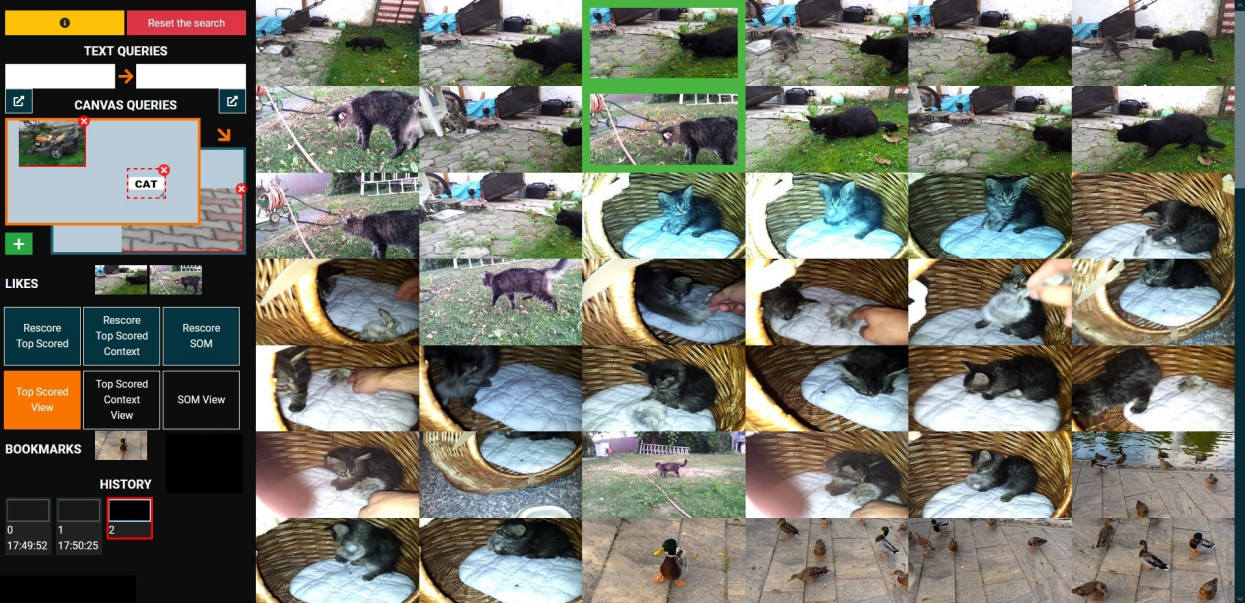
\includegraphics[width=0.8\textwidth]{content/resources/images/SOMHunter21.png}
    \caption{The interface of SOMHunter \cite{lokoc_enhanced_2021}. It is packed with features, which makes it a strong tool in the hands of an expert, however the interface can be too complicated to a normal user. }
    \label{fig:SOMHunter}
\end{figure}

System developers employ different user interaction modes to enable fast and effective data browsing. The most common form is a text bar with a gallery of results, as popularized by vitrivr \cite{heller_vitrivr_2022}, the winner of the LSC'19. This approach is also adopted, possibly with modifications by LifeSeeker \cite{nguyen_lifeseeker_2022}, FIRST \citeown{hoang-xuan_flexible_2022} and Myscéal \cite{tran_e-mysce_2022} with good results. As an example, Myscéal, the winner of the three most recent editions, besides showing the relevant images, automatically selects two more images before and after that image to preserve the temporal information of the moment. This allows users to have a quick glance over the preceding and succeeding moment, maintaining the logical flow of events. 

Other systems take interaction to another level by applying advanced visualization methods such as projection, or even virtual reality. To leverage the intuitive human perception of three-dimensional vision, PhotoCube \cite{shin_photocube_2021} proposed to project the high-dimensional data to just three dimensions, based on the Multidimensional Media Model ($M^3$). On the other hand, vitrivr-VR \cite{spiess_multimodal_2022}, with vitrivr \cite{heller_vitrivr_2022} as the underlying core, augments it with a virtual reality interface, in which users can input queries and browse through the data without being limited by a screen's area. ViRMA \cite{duane_virma_2021} combines $M^3$ and virtual reality to create an immersive searching experience centered around the user exploring the data and choosing the dimension to project on. Though these systems promote the visualization of the data, they have a slower user input time than conventional keyboard-and-screen systems. Coupled with the sheer size and the effectiveness of vision-language models and databases in the LSC, these methods often achieve inferior results on the benchmark.

\subsection{Previous versions}
\label{sec:previous_versions}

\begin{figure}
    \centering
    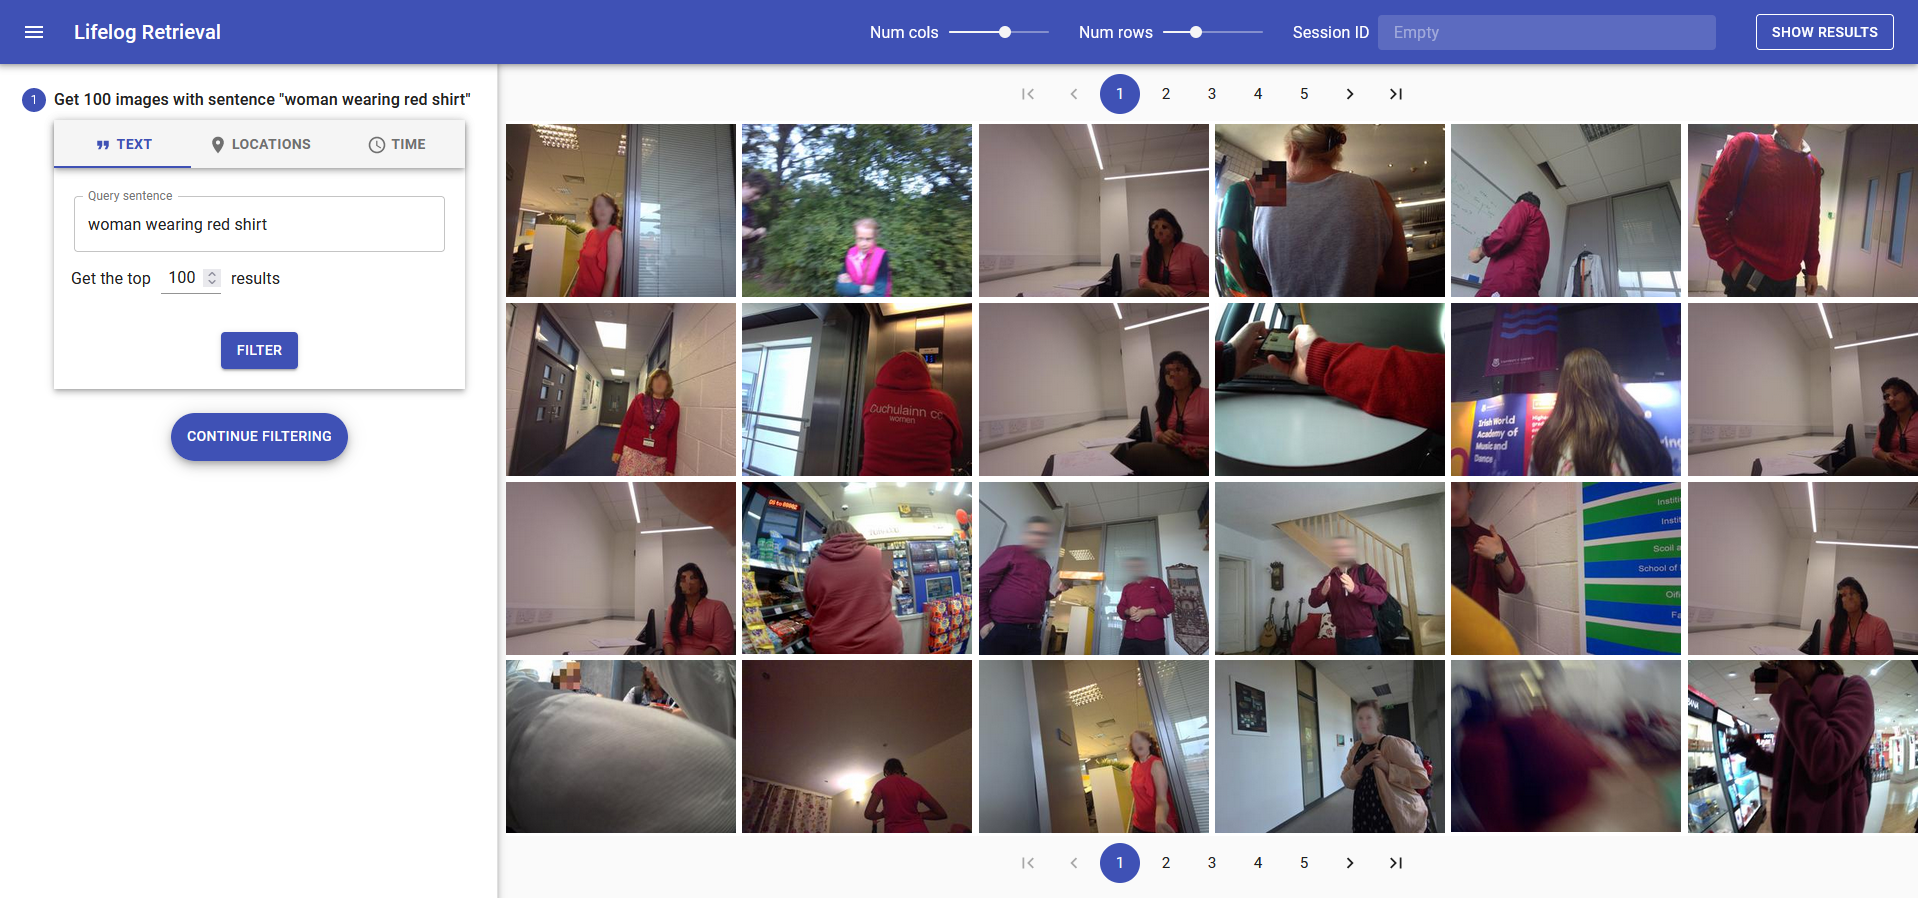
\includegraphics[width=0.8\textwidth]{content/resources/images/FIRST2.png}
    \caption{The interface of the previous version, FIRST 2.0 \cite{trang-trung_flexible_2021}}
    \label{fig:first2}
\end{figure}

The current system, FIRST 3.0 \citeown{hoang-xuan_flexible_2022}, is developed from the previous versions. As with other teams, throughout several years of participation in challenges, new ideas and lessons have been learned and integrated into the system. It has traditionally employed common space embeddings as the core retrieval method. The first version \cite{tran_first_2020}, which featured at LSC'20, used an autoencoder-like approach to map query text and image to a common feature space. As with contemporary methods, FIRST used separate encoders for textual and visual data, namely BERT \cite{devlin_bert_2019} and ResNet \cite{he_deep_2016}. This approach already allows free-form query sentences, e.g., "using cellphone in a train". In FIRST 2.0 \cite{trang-trung_flexible_2021}, the Self-Attention based Joint Embedding Model \cite{trang-trung_lifelog_2020} was used, which features the newer Transformer \cite{devlin_bert_2019} architecture and Transformer-based model. The second version also came with improvements in user interface and metadata processing, which is important for the user. Its interface is visible in Figure \ref{fig:first2}.

FIRST 3.0 \citeown{hoang-xuan_flexible_2022} builds on the success of previous versions and introduces zero-shot joint-embedding trained CLIP \cite{radford_learning_2021}, eliminating the need to adapt two separate models to the same domain. Furthermore, CLIP's flexibility enables simple implementation of features such as visual similarity search and query expansion. Furthermore, FIRST 3.0 features novel user interface features and a set of guidelines on how to best use the system.